% Created 2019-11-19 Tue 23:51
% Intended LaTeX compiler: pdflatex
\documentclass[presentation]{beamer}
\usepackage[utf8]{inputenc}
\usepackage[T1]{fontenc}
\usepackage{graphicx}
\usepackage{grffile}
\usepackage{longtable}
\usepackage{wrapfig}
\usepackage{rotating}
\usepackage[normalem]{ulem}
\usepackage{amsmath}
\usepackage{textcomp}
\usepackage{amssymb}
\usepackage{capt-of}
\usepackage{hyperref}
\institute{Universidad Nacional Autónoma de México}
\usetheme{metropolis}
\usecolortheme{}
\usefonttheme{}
\useinnertheme{}
\useoutertheme{}
\author{Adrián Antonio Rodríguez Pié}
\date{21 de noviembre de 2019}
\title{Implementación de redes neuronales convolucionales para el meta-análisis de acoplamientos moleculares de complejos proteína-ligando}
\AtBeginSection{\frame{\sectionpage}}
\metroset{block=fill}
\hypersetup{
 pdfauthor={Adrián Antonio Rodríguez Pié},
 pdftitle={Implementación de redes neuronales convolucionales para el meta-análisis de acoplamientos moleculares de complejos proteína-ligando},
 pdfkeywords={},
 pdfsubject={},
 pdfcreator={Emacs 27.0.50 (Org mode 9.1.9)},
 pdflang={English}}
\begin{document}

\maketitle
\begin{frame}{Outline}
\tableofcontents
\end{frame}



\section{Sobre proteínas}
\label{sec:org3dd8f81}
\begin{frame}[label={sec:org4b3872c}]{Proteínas}
\begin{block}{Orígen}
Originado del griego \emph{proteios} que significa "primario"
o "de primer orden".
\pause
\end{block}
\begin{block}{Definición (según la \alert{RAE})}
Sustancia constitutiva de la materia viva, formada
por una o varias cadenas de aminoácidos.
\end{block}
\end{frame}
\begin{frame}[label={sec:orga8db543}]{Ligandos}
\begin{itemize}
\item Un \alert{ligando} es una molécula que se une a otra molécula específica, en algunos casos mandando una señal en el proceso.
\pause
\item Estos ligandos interactuan con moleculas objetivo (usualmente otras proteínas). Son a estas proteínas a las que llamamos \alert{receptores} o \alert{residuos}.
\end{itemize}
\end{frame}
\begin{frame}[label={sec:org0f7604e}]{Docking}
\begin{block}{Acoplamiento molecular}
Método cuyo objetivo es predecir los estados tanto estructurales,
llamadas \alert{poses}, como energéticos, prediciendo la afinidad del enlace
entre moléculas.
\begin{center}
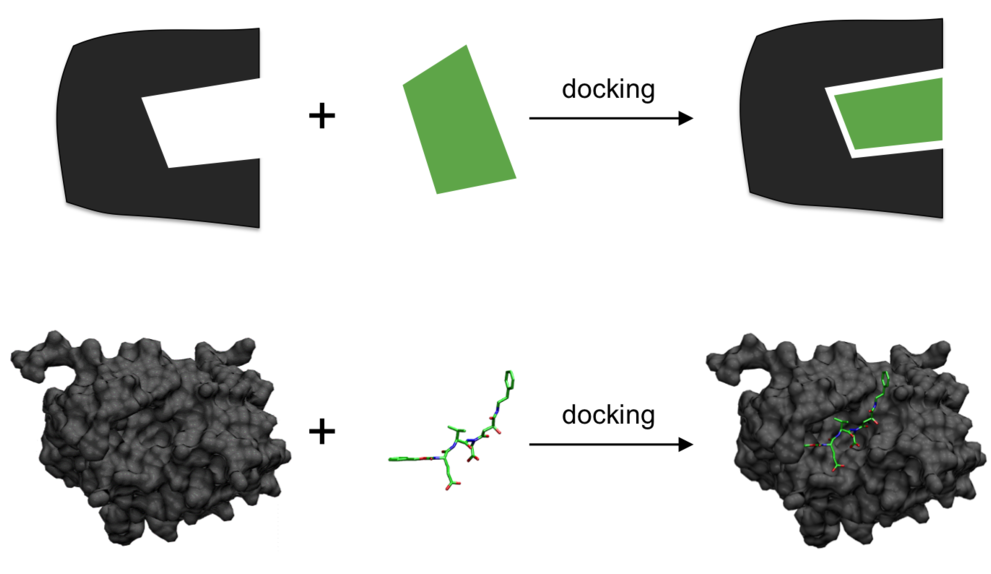
\includegraphics[width=.9\linewidth]{images/docking.png}
\end{center}
\end{block}
\end{frame}
\begin{frame}[label={sec:org0d747d5}]{Pasos del docking}
\begin{center}
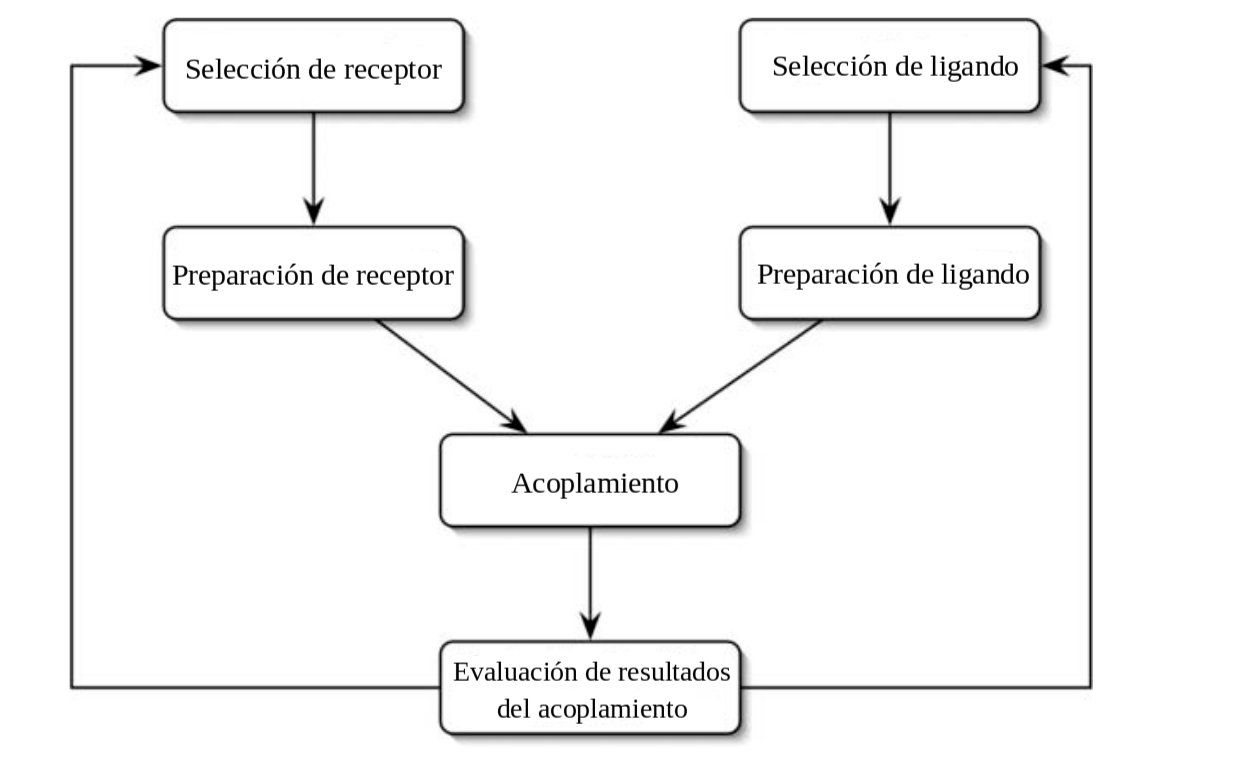
\includegraphics[width=.9\linewidth]{images/docking_steps.png}
\end{center}
\end{frame}
\section{Sobre inteligencia artificial}
\label{sec:org3f383da}
\begin{frame}[label={sec:org13fc64d}]{La prueba de Turing}
\begin{center}
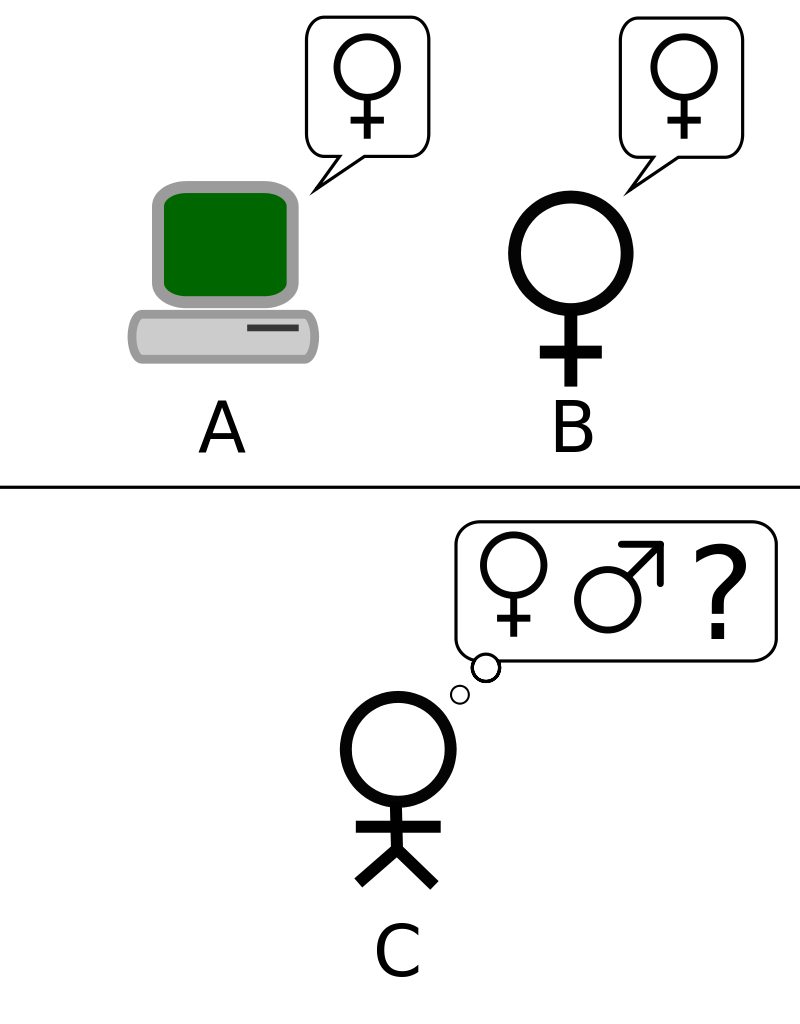
\includegraphics[width=170px]{images/turing-test.png}
\end{center}
\end{frame}
\begin{frame}[label={sec:org409b652}]{IA y agentes}
\begin{block}{Inteligencia artrificial}
\alert{\alert{Agentes racionales}} que, mediante \alert{\alert{sensores}}, pueden
percibir su \alert{\alert{entorno}} y actuar sobre él a partir de un
sistema de decisión.
\pause
\end{block}
\begin{block}{Agentes}
Máquina compuesta por un conjunto finito de estados, cuyas
transiciones están dadas por reglas de inferencias.
\end{block}
\end{frame}
\section{Sobre redes y neuronas}
\label{sec:orgccbd527}
\begin{frame}[label={sec:org3a7f611}]{Inspiración en la biología}
\begin{center}
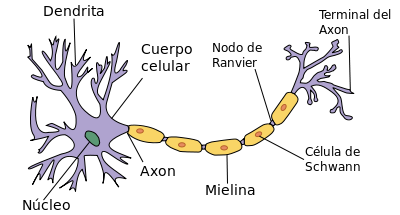
\includegraphics[width=.9\linewidth]{images/neurona.png}
\end{center}
\end{frame}

\begin{frame}[label={sec:orgea486d3}]{El perceptrón}
\begin{block}{Definiciónes}
\begin{itemize}
\item \alert{x} \(\in \mathbb{R}^n\) (muestra)
\item \alert{w} \(\in \mathbb{R}^n\) (vector de pesos)
\item \alert{\(\theta\)} \(\in \mathbb{R}^n\) (umbral de activación)
\item \alert{y} \(\in \{0, 1\}\) (valor real de la muestra)
\item \alert{\(\hat y\)} \(\in \{0, 1\}\) (valor predicho de la muestra)
\end{itemize}
Por último, definimos \alert{z} como una combinación líneal de \alert{x} y \alert{w}
\(z=w_1x_1+...w_nx_n\) \\
Llamamos a \alert{z} la \emph{entrada de la red}.
\pause
\end{block}
\begin{block}{Función de activación}
Definimos
\begin{equation*}
\phi(z)= \left\{ \begin{array} {rl} 1 & \text{si } z \geq \theta
\\ -1 & \text{en otro caso} \end{array} \right.
\end{equation*}
\end{block}
\end{frame}

\begin{frame}[label={sec:org47bafc0}]{Pasos del perceptrón}
\begin{enumerate}
\item Inicializar los pesos en cero o en números aleatorios cercanos a cero.
\end{enumerate}
\pause
\begin{enumerate}
\item Para cada muestra de entrenamiento \(x\), realizar lo siguiente:
\end{enumerate}
\pause
a) Calcular el valor de salida \(\hat y\) (\(\hat y = \phi(z)\)).\\
\pause
b) Actualizar los pesos en \(w\) a partir del error \(\Delta w\).

Con \(\Delta w\) dado por:
\begin{equation*}
\Delta w = \eta (y - \hat y)x
\end{equation*}

Donde \(\eta \in [0,1]\) es el \emph{índice de aprendizaje}.
\end{frame}

\begin{frame}[label={sec:orga4e94aa}]{Diagrama del perceptrón}
\begin{center}
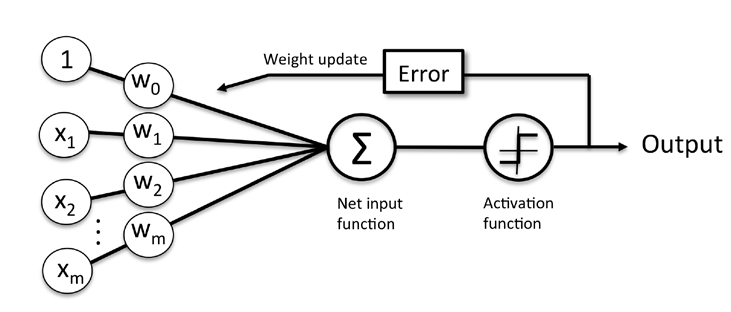
\includegraphics[width=.9\linewidth]{images/perceptron-summary.png}
\end{center}
\end{frame}

\begin{frame}[label={sec:org3d2b48a}]{El perceptrón multicapa}
\begin{center}
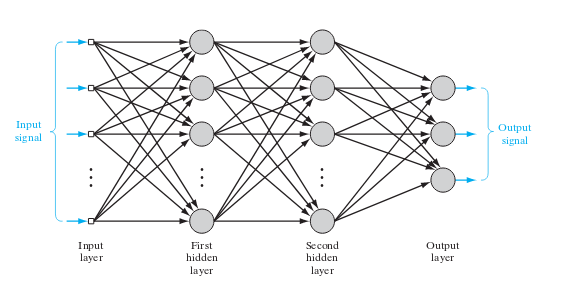
\includegraphics[width=.9\linewidth]{images/mlp.png}
\end{center}
\end{frame}
\begin{frame}[label={sec:orgd4aec04}]{El perceptrón multicapa}
\begin{center}
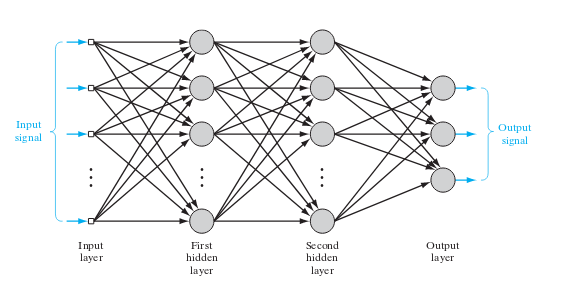
\includegraphics[width=170px]{images/mlp.png}
\end{center}
\begin{block}{Función de costo o error}
Definimos la función de costo \alert{\(J\)} para el perceptrón multicapa
como la suma de los errores cuadrados entre la salida calculada y
el valor real:
\begin{equation*}
J(w)=1/2n \sum_{i=1}^n (\hat{y}_i - y_i^2)
\end{equation*}

\pause
\begin{center}
¡Es diferenciable!
\end{center}
\end{block}
\end{frame}
\begin{frame}[label={sec:orgb7b2257}]{Descenso por el gradiente}
\begin{center}
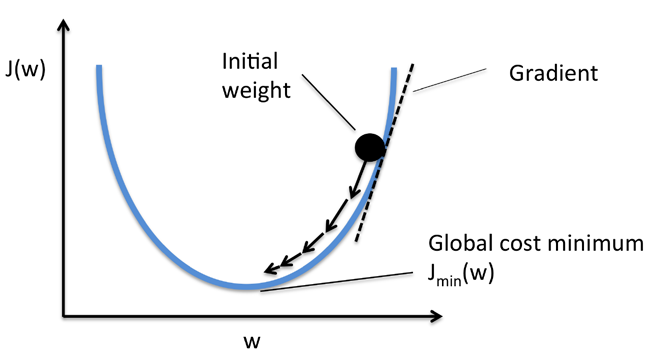
\includegraphics[width=.9\linewidth]{images/gradient-descent.png}
\end{center}
\end{frame}

\section{Sobre meta-análisis del acoplamiento}
\label{sec:orgf5e6a0c}
\begin{frame}[label={sec:org9bd933f}]{Preparación de la base de datos}
\pause
\begin{enumerate}
\item Se filtran las proteínas que no contengan ligandos.
\pause
\item Se eliminan todas las proteínas con peso molecular menor a 300 Da.
\pause
\item Se filtran de las proteínas las cadenas de ADN y ARN.
\pause
\item Se quitan también los metales pesados de las proteínas.
\end{enumerate}
\end{frame}
\begin{frame}[label={sec:orga2cd831}]{Preparación de la base de datos}
\begin{enumerate}
\setcounter{enumi}{4}
\item Se definen las cargas de la proteína, así como sus libertades de torsión (\alert{ramas}).
\pause
\begin{center}
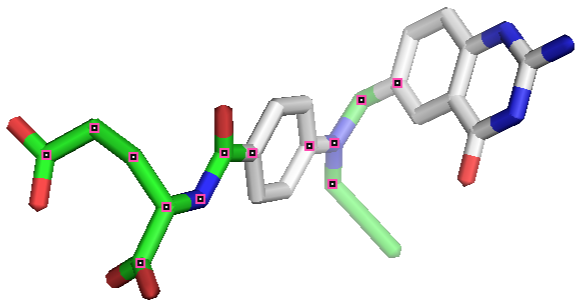
\includegraphics[width=.9\linewidth]{images/torsions.png}
\end{center}
\end{enumerate}
\end{frame}
\begin{frame}[label={sec:org0e730a6}]{Preparación de la base de datos}
\begin{enumerate}
\setcounter{enumi}{5}
\item Se separa cada par proteína-ligando.
\pause
\item Se hace el acoplamiento virtual de cada par.
\pause
\begin{center}
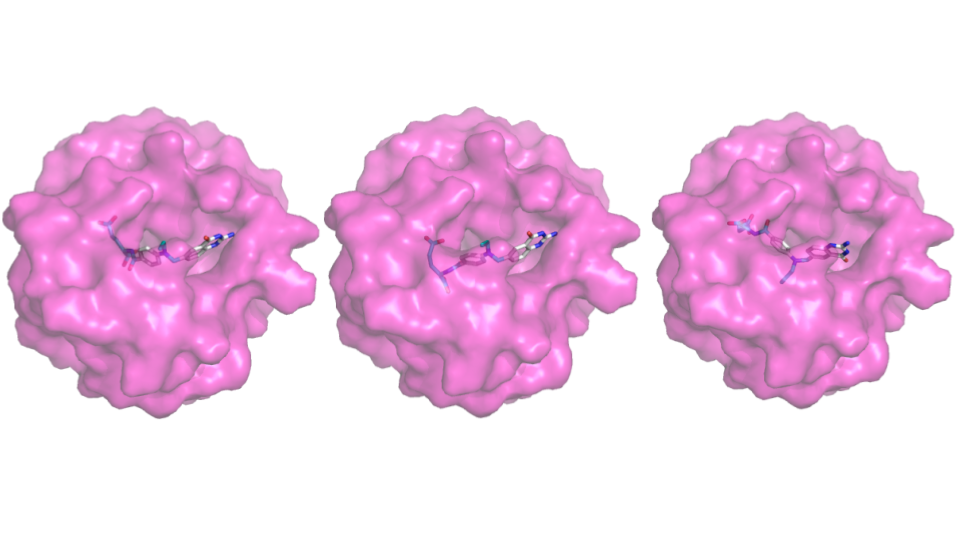
\includegraphics[width=.9\linewidth]{images/poses.png}
\end{center}
\end{enumerate}
\end{frame}
\begin{frame}[label={sec:org6336f08}]{Preparación de la base de datos}
Se genera entonces un listado de poses con una calificación asociada, que
se compara con el RMSD del compuesto cristalográfico original.
\pause
\begin{table}[H]
\begin{tabular}{|c|c|c|c|}
\hline
Pose         & \begin{tabular}[c]{@{}c@{}}Clasificación\\ (según AutoDock Vina)\end{tabular} & Calificación & RMSD  \\ \hline
4EIL\_CB3\_A\_1 & 1                                                                             & -10.2        & 3.08  \\
4EIL\_CB3\_A\_2 & 2                                                                             & -10.0         & 3.02  \\
4EIL\_CB3\_A\_3 & 3                                                                             & -9.8         & 3.02  \\
4EIL\_CB3\_A\_4 & 4                                                                             & -9.5         & 1.31  \\
4EIL\_CB3\_A\_5 & 5                                                                             & -9.3         & 3.0  \\ \hline
\end{tabular}
\end{table}
\end{frame}

\begin{frame}[label={sec:org858f579}]{Deep-pose}
\begin{block}{Deep-pose}
Una red neuronal convolucional profunda que toma la información de
un acomplamiento en un complejo proteína-ligando como entrada y
produce una calificación de qué tan viable es dicha pose.
\begin{center}
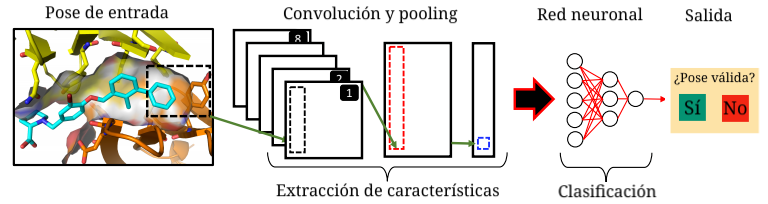
\includegraphics[width=.9\linewidth]{images/architecture.png}
\end{center}
\end{block}
\end{frame}
\section{Deep-pose}
\label{sec:orgf3e7538}
\begin{frame}[label={sec:org6ca578b}]{Contexto de la rama}
\pause
\begin{block}{Codificación del contexto de la rama}
SMILES (\emph{Simple Molecular Input Line Entry System}) es un sencillo
lenguaje químico que permite describir moléculas utilizando únicamente
caracteres ASCII.
\pause
\begin{itemize}
\item Es sumamente compacta.
\pause
\item Es canónica.
\end{itemize}
\end{block}
\end{frame}
\begin{frame}[label={sec:org200f255}]{Diccionarios de ramas}
\pause
\begin{center}
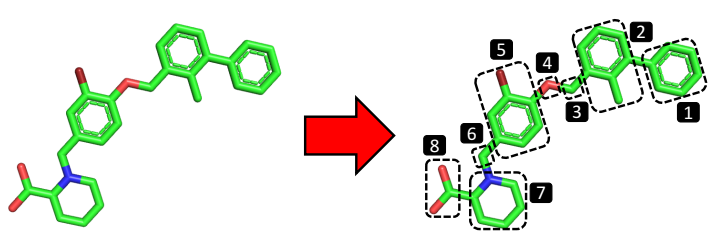
\includegraphics[width=.9\linewidth]{images/branches.png}
\end{center}
\pause
\begin{block}{Diccionarios de ramas}
\begin{itemize}
\item Se enlistan todas las ramas codificadas distintas y a cada una se
le asigna un índice (\alert{diccionario de ramas}).
\item Se segmentan los rangos de distancias entre ramas encontrados
en compartimentos, y a cada uno de estos se le asigna también un
índice (\alert{diccionario de distancias}).
\end{itemize}
\end{block}
\end{frame}

\begin{frame}[label={sec:orgaa8eb44}]{Fragmento de los diccionarios de ramas y de distancias}
\begin{table}[H]
  \begin{center}
    \begin{tabular}{l|l}
      SMILES                 & Idx \\ \hline
      NC1=N{[}C{]}(=NC=C1)=O & 93 \\
      C1CCCCC1               & 94 \\
      CNC=O                  & 95 \\
      NC=N                   & 96 \\
      CC=C                   & 97
    \end{tabular}
    \begin{tabular}{l|l}
      Rango de distancia (\AA) & Idx \\ \hline
      3.0526 - 3.2631        & 6   \\
      3.2632 - 3.4736        & 7   \\
      3.4737 - 3.6842        & 8   \\
      3.6843 - 3.8947        & 9   \\
      3.8948 - 4.1052        & 10
    \end{tabular}
  \end{center}
\end{table}
\end{frame}
\begin{frame}[label={sec:orgc2f7152}]{Codificación del contexto de la rama}
Para cada rama del ligando, se codifican entonces las cinco
ramas más cercanas del receptor a través de sus tipos y sus distancias.
\pause
\begin{block}{Traducción de la rama \alert{OP(O)O} en una tupla.}
\pause
\begin{table}[H]
  \begin{center}
  \begin{tabular}{l|l}
    Ramas cercanas a OP(O)O & Distancia en \AA \\ \hline N & 5.794664 \\ C1CC1 & 5.691862
    \\ NC1=N{[}C{]}(=NC=C1)=O & 4.449922 \\ NC=N & 3.785496 \\ O &
    3.747894
  \end{tabular}
  \end{center}
\end{table}
\pause
\begin{equation*}
\downarrow
\end{equation*}
\begin{equation*}
  OP(O)O=\begin{bmatrix}
  (2, 13, 93, 96, 4) & (11, 10, 7, 4, 4)
  \end{bmatrix}
\end{equation*}
\end{block}
\end{frame}

\begin{frame}[label={sec:orgec87ae7}]{Representación vectorial del contexto de la rama}
\begin{block}{Definiciones}
\begin{itemize}
\item \alert{\(B\)} El conjunto de tipos de ramas.
\item \alert{\(N\)} Dimensión de los vectores característicos (\alert{hiperparámetro}).
\item \alert{\(W^{b\_type}\)} \(\in \mathbb{R}^{N\times |B|}\).
\end{itemize}
\end{block}
\end{frame}

\begin{frame}[label={sec:org95d6516}]{Representación vectorial del contexto de la rama}
  \begin{table}[H]
    \begin{equation*}
      Rama=\begin{bmatrix}
      OP=O, & OC=O, & C=O, & OPO, & OP=O
      \end{bmatrix}
    \end{equation*}
    \begin{center}
      $W_{b\_type}$
      \begin{tabular}{|l|l|l|l|l|l|l|}
    	\hline
    	OP=O & OC=O & OPO & C=O & NC=O & OPO & OP=O \\ \hline
    	&      &     &     &      &     &      \\ \hline
    	&      &     &     &      &     &      \\ \hline
    	&      &     &     &      &     &      \\ \hline
      \end{tabular}
    \end{center}
  \begin{equation*}
  \downarrow
  \end{equation*}
  \begin{equation*}
    z_{b\_type}^T =
  \begin{tabular}{lllllllllllllll}
\multicolumn{3}{l}{OP=O}                                               &                       & \multicolumn{3}{l}{OC=O}                                              &                       & \multicolumn{3}{l}{C=O}                                               &                       & \multicolumn{3}{l}{OPO}                                               \\ \cline{1-3} \cline{5-7} \cline{9-11} \cline{13-15}
\multicolumn{1}{|l|}{} & \multicolumn{1}{l|}{} & \multicolumn{1}{l|}{} & \multicolumn{1}{l|}{$\bullet$} & \multicolumn{1}{l|}{} & \multicolumn{1}{l|}{} & \multicolumn{1}{l|}{} & \multicolumn{1}{l|}{$\bullet$} & \multicolumn{1}{l|}{} & \multicolumn{1}{l|}{} & \multicolumn{1}{l|}{} & \multicolumn{1}{l|}{$\bullet$} & \multicolumn{1}{l|}{} & \multicolumn{1}{l|}{} & \multicolumn{1}{l|}{} \\ \cline{1-3} \cline{5-7} \cline{9-11} \cline{13-15}
  \end{tabular}
  \end{equation*}
  \end{table}
\end{frame}
\begin{frame}[label={sec:org6e1ad69}]{Representación vectorial del contexto de la rama}
Analogamente se genera el vector \(z_{b\_dist}\).
\pause
\begin{block}{Representación del contexto de la rama}
Finalmente, la representación del contexto de la rama \(b\) se define como
\begin{equation*}
z_b = z_{b\_type} \bullet z_{b\_dist}
\end{equation*}
\end{block}
\end{frame}

\begin{frame}[label={sec:org7456708}]{Representación de la pose de un complejo proteina-ligando}
La entrada de la capa convolucional es una lista de vectores
\(\{z_1, z_2, ..., z_n\}\) donde \(z_i\) es la representación vectorial
del contexto de la \(i\)-ésima rama del ligando.
\pause
\begin{block}{Primera etapa de la capa convolucional (extracción de características)}
\begin{equation*}
  u_i = f(z_i + b^{conv})
\end{equation*}
donde:
\begin{itemize}
\item \(f\) es la función tangente hiperbólica.
\item \(b^{conv}\) es el sesgo.
\end{itemize}
\pause
\end{block}
\begin{block}{Segunda etapa de la capa convolucional \emph{(max-pooling)}}
\begin{equation*}
  [r]_j = \max_{1 \leq i \leq n} [u_i]_j
\end{equation*}
\end{block}
\end{frame}

\begin{frame}[label={sec:org09a8f24}]{Clasificación de la pose}
Finalmente el vector \(r\) es procesado por dos capas neuronales más:
\begin{enumerate}
\item Una tercera capa oculta que reprsenta un nivel más de abstracción.
\item Una última capa de salida donde se dá la clasificación.
\end{enumerate}

Es en esta última capa donde se computa una calificación para cada
una de las posibles clasificaciónes de la pose: (0) pose \alert{señuelo} y
(1) pose \alert{válida}.
\end{frame}
\begin{frame}[label={sec:org53ad36c}]{Arquitectura de la red}
\begin{center}
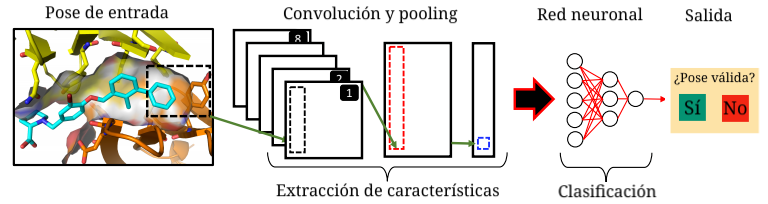
\includegraphics[width=.9\linewidth]{images/architecture.png}
\end{center}
\end{frame}
\section{Entrenamiento y resultados}
\label{sec:orgebe02e0}
\begin{frame}[label={sec:orgc40c9e5}]{Hiperparámetros}
\begin{table}[H]
\begin{center}
\begin{tabular}{|c|c|c|}
\hline
Hiperparámetro & Descripción                         & Valor \\ \hline
\textit{N}     & Dimensión del vector característico & 80    \\
\textit{cf}    & Unidades en la capa convolucional   & 150   \\
\textit{h}     & Unidades en la capa oculta          & 60    \\
\textit{bs}    & \textit{Tamaño de los minilotes}    & 20    \\
$\lambda$         & Índice de aprendizaje               & 0.1   \\ \hline
\end{tabular}
\end{center}
\end{table}
\end{frame}

\begin{frame}[label={sec:org42ebe9b}]{Calibración de hiperparámetros}
\begin{center}
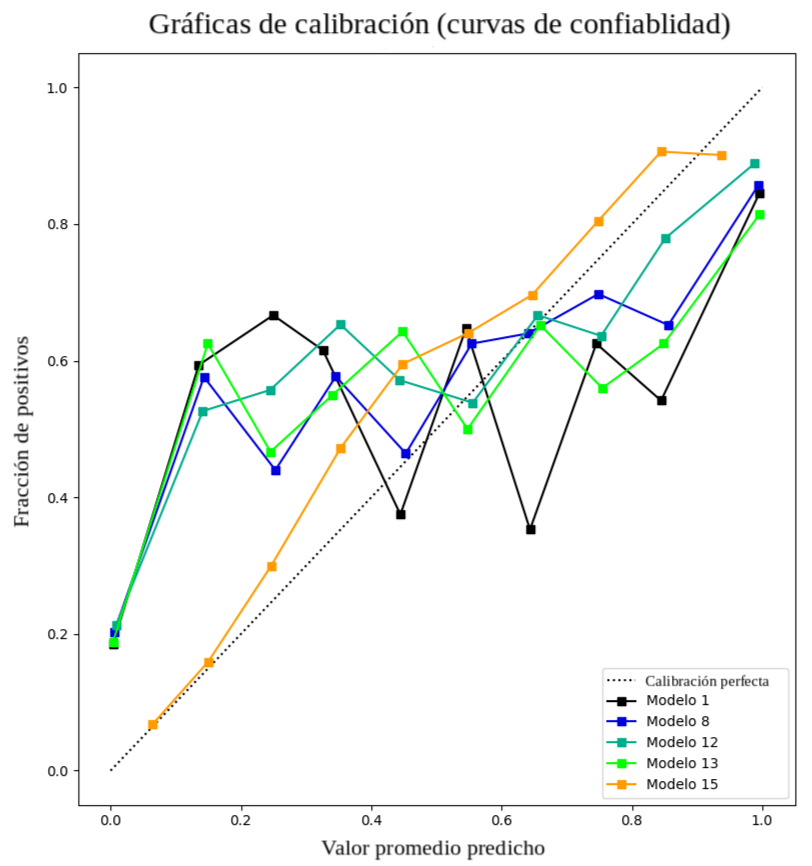
\includegraphics[width=190px]{images/calibration.png}
\end{center}
\end{frame}
\begin{frame}[label={sec:orgc0d703b}]{Resultados}
\begin{center}
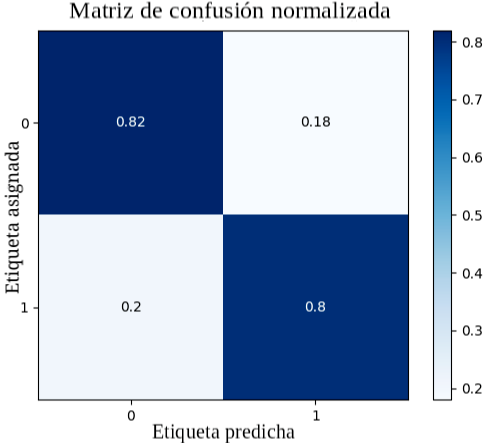
\includegraphics[width=190px]{images/confusion.png}
\end{center}
\end{frame}

\section{¿Preguntas?}
\label{sec:org7391999}
\end{document}
